\documentclass[xcolor={dvipsnames,svgnames}]{beamer}
\usetheme{PaloAlto}
\usecolortheme{spruce}
\usepackage[english]{babel}
\usepackage[utf8]{inputenc} % Required for inputting international characters
\usepackage[T1]{fontenc} % Output font encoding for international characters
% \usepackage{subcaption}
\usepackage{mathpazo} % Use the Palatino font by default
\usepackage{booktabs}
\usepackage{amssymb}
\usepackage{colortbl}
\usepackage[final]{pdfpages}
\usepackage{xcolor}
\usepackage{balance}
\usepackage{epigraph}
\usepackage{alltt} % for code snippet
\usepackage{listings}
\usepackage{hyperref}
\usepackage{amsmath}
\usepackage{macros}
\usepackage{mathtools}
\usepackage{float}
\usepackage{newtxmath}
\usepackage{polski}
\usepackage{bbm}
\usepackage{tikz-cd}
\usepackage{flowchart}
\usepackage{tabularx}
\usepackage{array}
\setlength\extrarowheight{2pt}
\usepackage[mathscr]{euscript}
\usetikzlibrary{
  shapes,
  arrows.meta, % supersedes arrows
  calc,automata,positioning,fit,quotes}
  \tikzset{
  line/.style={draw, -Latex}
}
\tikzstyle{arrow} = [thick,->,>=stealth]
\DeclareMathOperator{\Cech}{\check{C}}
\usepackage[backend=bibtex,style=authoryear,natbib=true]{biblatex} % Use the bibtex backend with the authoryear citation style (which resembles APA)
%\usepackage[backend=bibtex,style=authoryear,natbib=true,backref=true]{biblatex} % use this line instead of the previous one if you want to use back references
\usepackage{caption}
\usepackage{subcaption}
\captionsetup{font=normalsize,labelfont={bf,sf}}
\captionsetup[subfigure]{font=scriptsize,labelfont=scriptsize}
% \usepackage{subfig, graphicx}

\makeatletter
  \setbeamertemplate{sidebar \beamer@sidebarside}%{sidebar theme}
  {
    \beamer@tempdim=\beamer@sidebarwidth%
    \advance\beamer@tempdim by -6pt%
    \insertverticalnavigation{\beamer@sidebarwidth}%
    \vfill
    \ifx\beamer@sidebarside\beamer@lefttext%
    \else%
      \usebeamercolor{normal text}%
      \llap{\usebeamertemplate***{navigation symbols}\hskip0.1cm}%
      \vskip2pt%
    \fi%
}%

\addbibresource{biblio.bib}

\title{$p$-Wasserstein Distance between High-Dimensional Point Clouds \\ via Persistent Homology}
\author{Zhang Liu\\ Supervisor: Prof.~Han Fei}

\date{Novemember 15, 2021}

\begin{document}
\section{Introduction}
\begin{frame}
\titlepage
\end{frame}
\begin{frame}{Research background: topological data analysis (TDA)}
\begin{itemize}
    \item ``Topological'': to extract, analyze and make use of the topological and geometric structures underlying data
    \item ``Data'': high-dimensional point clouds = metric spaces
    \item Topological features capture the global structure of the data and provide useful information on the connectedness and clusters
    \item \textbf{How can high-dimensional point clouds be compared based on their topological structures?}
\end{itemize}
\end{frame}

\begin{frame}{Project Overview}
    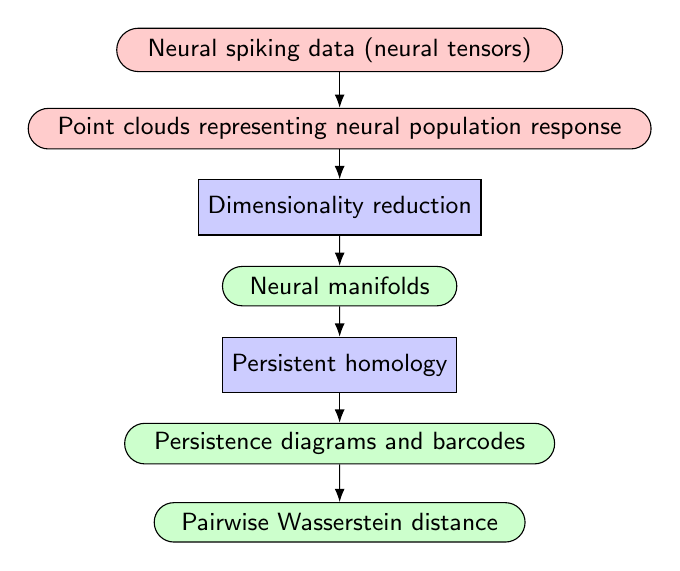
\begin{tikzpicture}[font={\sf \small}]
 \def\smbwd{2cm}
%   \node (BNN) at (-3,0.5) [draw, terminal, minimum width=\smbwd,  fill=yellow!20, minimum height=0.5cm] {Biological Neural Networks}; 
%   \node (ANN) at (2.7,0.5) [draw, terminal, minimum width=\smbwd,  fill=yellow!20, minimum height=0.5cm] {Artificial Neural Networks}; 
  %------------
  \node (experimental) at (1.5,0) [draw, terminal, minimum width=\smbwd,  fill=red!20, minimum height=0.5cm]{Neural spiking data (neural tensors)};
%   \node (artificial) at (2.7,-1)[draw, terminal,minimum width=\smbwd,  fill=red!20, minimum height=0.5cm]{neuron output (simulations)};
  %------------
  \node (tensors) at (1.5,-1) [draw, terminal, minimum width=\smbwd,  fill=red!20, minimum height=0.5cm] {Point clouds representing neural population response}; 
  %------------
  
  \node (diffusion) at (1.5,-2) [draw, process, minimum width=\smbwd, fill=blue!20, minimum height=0.7cm] {Dimensionality reduction};
  %------------
  
  \node (manifolds) at (1.5,-3) [draw, terminal, minimum width=\smbwd,  fill=green!20, minimum height=0.5cm] {Neural manifolds};
  
   \node (persistent) at (1.5,-4) [draw, process, minimum width=\smbwd, fill=blue!20, minimum height=0.7cm] {Persistent homology};
   
   \node (features) at (1.5,-5) [draw, terminal, minimum width=\smbwd,  fill=green!20, minimum height=0.5cm] {Persistence diagrams and barcodes};
   
   \node (wasserstein) at (1.5,-6) [draw, terminal, minimum width=\smbwd,  fill=green!20, minimum height=0.5cm] {Pairwise Wasserstein distance};
  
  %------------
  
%  \path [line](BNN) -- (experimental);
%  \path [line](ANN) -- (artificial);
 \path [line](tensors) -- (diffusion);
 \path [line](experimental) -- (tensors) ;
%  \path [line] (artificial) -- (tensors) ;
 \path [line](diffusion) -- (manifolds);
  \path [line](manifolds) -- (persistent);
   \path [line](persistent) -- (features);
  \path [line](features) -- (wasserstein); 
 \end{tikzpicture}
\end{frame}

% -----------------------------------------------
\section{Persistent Homology}
\begin{frame}{Advantages of TDA}
    The major advantages for using TDA to analyze high-dimensional point clouds:
\begin{enumerate}
	\item TDA provides qualitative information which is required for data analysis.
	
	\item Compared to straightforward geometric methods, TDA is less sensitive to the actual choice of metrics. 
	
	\item Studying geometric objects using TDA does not depend on the coordinates. 
	\end{enumerate}
\end{frame}

\begin{frame}{Simplicial complex}
    
\begin{defn}[Simplicial complex]
	An \underline{abstract simplicial complex} is a pair $(V, \triangle)$, where $V$ is a finite set, and $\triangle$ is a family of non-empty subsets of $V$ such that 
	\begin{align}
	    \tau \in \triangle \text{ and }\sigma \subseteq \tau \implies \sigma \in \triangle.
	\end{align}
	$\tau \in \triangle $ is face of $\triangle$. The dimension of a face $\tau$ is $|\tau| - 1.$
	\end{defn}

	(Intuition) A simplicial complex $\triangle$ in $\mathbb{R}^n$ is a collection of simplices in $\mathbb{R}^n$ such that
	\begin{enumerate}
	    \item Every face of a simplex of $\triangle$ is in $\triangle$.
	    \item The intersection of any two simplicies of $\triangle$ is a face of each. 
	\end{enumerate}
\end{frame}

\begin{frame}{An example of a simplicial complex}
Suppose the family of sets 
    $$\emptyset, \{a\},\{b\},\{c\}, \{d\}, \{a,b\}, \{a,c\}, \{b,c\}, \{b,d\}, \{c,d\}, \{a,b,c\}$$ form a simplicial complex $E_1$.
\begin{figure}[H]
        \centering 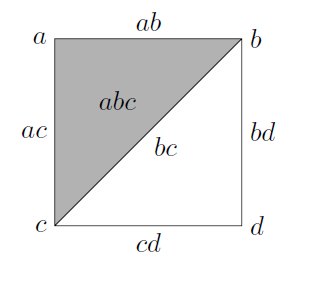
\includegraphics[width=0.4\textwidth]{figures/E1.png}
            \caption{Geometric realizatoin of the simplicial compelx $E_1$.}
    \end{figure}
\end{frame}


\begin{frame}{Simplicial chain complex}
\begin{defn}[Simplicial chain complex]
The \underline{simplicial chain complex} of a simplicial comlex $\triangle$, denoted with $C(\triangle)$, is defined as:
\begin{figure}[H]
        \centering 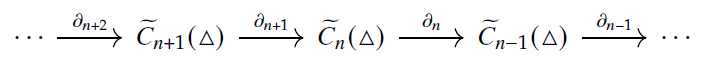
\includegraphics[width=0.8\textwidth]{figures/chain.png}
    \end{figure}
\end{defn}
The simplicial chain complex of $E_1$,  $C(E_1)$ is 
\begin{figure}[H]
        \centering 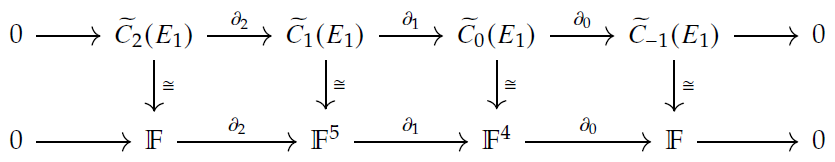
\includegraphics[width=0.8\textwidth]{figures/chain_E1.png}
    \end{figure}
\end{frame}

\begin{frame}{Simplicial homology of degree $k$}
    \begin{defn}[Simplicial homology of degree $k$]
\label{kth-homology-group}
    \begin{itemize}
        \item Cycle group, 
        
        $Z_k(\triangle; \mathbb{F}) = ker(\partial_k) = \{Z \in \Chain_k(\triangle; \FF): \partial_k(Z) = 0\}$ 
        \item Boundary group, 
        
        $B_k(\triangle;\FF) = im(\partial_{k+1}) = \{Z \in \Chain_k(\triangle; \FF): \partial_{k+1}(x), \quad x \in \Chain_{k+1}(\triangle; \FF)\}$ 
        \item \underline{Simplicial homology group} is the quotient group,
        \begin{align}
        \Hom_k(\triangle;\FF) &\coloneqq ker(\partial_k) / im(\partial_{k+1})\\
        &= Z_k(\triangle;\FF) / B_k(\triangle;\FF)
        \end{align}
    \end{itemize}
    %  $B_k(\triangle;\FF)\subseteq Z_k(\triangle;\FF) \subseteq C_k(\triangle;\FF)$
\end{defn}
    (Intuition) The simplicial homology gives an algebraic measure on the amount of cycles that are not the boundaries. 
\end{frame}

\begin{frame}{$k$-th Betti number}
    \begin{defn}[$k$-th Betti number]
\label{kth-betti}
    The \underline{$k$-th Betti number} of the simplicial complex $\triangle$ is
    \begin{align}
        \beta_k(\triangle;\FF) &\coloneqq \dim \Hom_k(\triangle;\FF) \\
        &= \dim ker(\partial_k) - \dim im(\partial_{k + 1}).
    \end{align}
    
    \begin{itemize}
        \item elements in $ker(\partial_k)$ are called $k$-cycles.
        \item elements in $im(\partial_k)$ are called $k$-boundaries.
        \item $k$-cycles that are not boundaries represent $k$-holes, which means that the $k$-th Betti number $\beta_k(\triangle; \FF)$ is the number of $k$-holes. 
    \end{itemize}
\end{defn} 
\end{frame}

\begin{frame}{An example for cycles and boundaries}
\begin{figure}[H]
   \label{matching}
        \centering 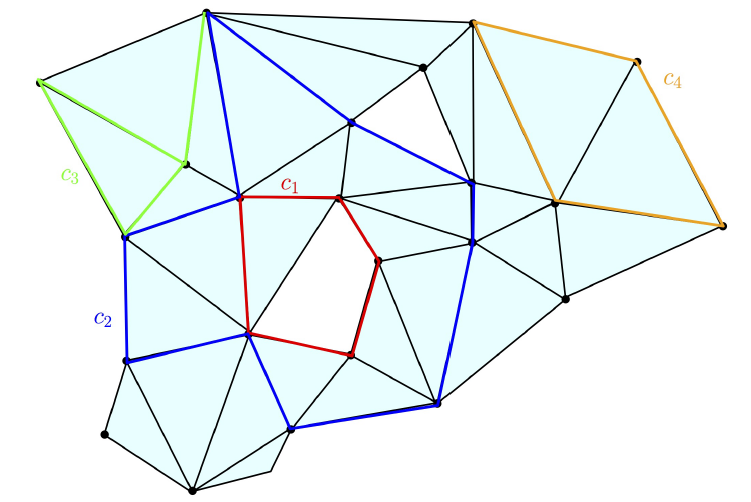
\includegraphics[width=0.6\textwidth]{figures/simplicial_complex.png}
            \caption{A $2$-dimensional simplicial complex $K$.}
    \end{figure}
\begin{itemize}
    \item $c_1, c2, c4$ are 1-cycles.
    \item $c_3$ is a 1-chain but not a 1-cycle.
    \item $c_4$ is the 1-boundary, namely the boundary
of the 2-chain obtained as the sum of the two triangles surrounded by $c_4$. 
\end{itemize}
\end{frame}

\begin{frame}{Persistent homology}
 
\begin{enumerate}
    \item The main idea of \textit{persistence}: from a fixed value of the threshold $\epsilon$ to all the different values of $\epsilon$ at once.
    \item As $\epsilon$ increases, we add simplicies to the complexes and detect which features ``persist."
    \item It is robust with regards to perturbations in the input data. 
\end{enumerate}
\end{frame}

\begin{frame}{$p$-persistent $k$-th homology group}
\begin{defn}[Filtered simplicial complex]
\label{filtered}
The simplicial complex $\triangle$ with such a sequence of subcomplexes, $\emptyset \subseteq \triangle^1 \subseteq \triangle^2 \subseteq \cdots \subseteq \triangle^m = \triangle$, is called \underline{filtered simplicial complex}.
\end{defn}
\begin{defn}[$p$-persistent $k$-th homology group]
Given a filtered complex, the \underline{$p$-persistent $k$-th homology group} $H_k^{i,p}$ of for the $i$-th subcomplex $\triangle^i$ is 
\begin{itemize}
    \item $H_k^{i,p} = Z_k^i / (B_k^{i+p}\cap Z_k^i)$
    % \item (equivalently) $H_k{i,p} \cong Im(\eta_k^{i,p})$, where $\eta_k^{i,p}$ is a bijection $\eta_k^{i,p}: H_k^i \to H_k^{i+p}$ that maps a homology class into another homology class containing it.   
\end{itemize}
\end{defn}
Note that this is simply the definition of homology group of degree $k$ in Definition \ref{kth-homology-group} with the additional notion of persistence.
\end{frame}

\begin{frame}{Classification Theorem}

\begin{thm}[Classification Theorem]
    For a finite persistence module $\mathscr{M}$ with coefficients in the field $F$, 
    \begin{equation}
        H_*(\mathscr{M}; F) \cong \underbrace{\bigoplus_i x^{t_i}F(x)}_\text{free module} \oplus  \underbrace{\left(\bigoplus_j x^{r_j}(F(x)/(x^{s_j}F[x]))\right)}_\text{torsion module}
    \end{equation}
    \end{thm}
    
    \begin{itemize}
        \item bijection between $\{$free elements$\}$ and $\{$homology generators with birth at $t_i$ and persist forever$\}$
       
       \item bijection between $\{$torsion elements$\}$  and  $\{$homology generators with birth at $r_j$ and death at $r_j + s_j\}$.
    \end{itemize}
\end{frame}

\begin{frame}{Barcode as the persistence analogue of Betti number}
\begin{itemize}
    \item The classification theorem gives the fundamental characterization of \textbf{persistence barcode}.
    \item $H_*^{i\to j}(\mathscr{C}^i_*; F)$ gives the number of intervals that contain $i$.
    \item As with Betti number, the barcode for $H_k$ does not give the actual structure of the homology group, but just a continuously parameterized rank. 
    \item The barcode is useful in that it can qualitatively filter out topological noise (since they are ``short-lived" features) and capture significant topological features (features that persist over increasing values of $\epsilon$).
\end{itemize}
\end{frame}


%------------------------------------------------
\section{Distances}
\begin{frame}{Distances between points in \RR^d: $L_p$ Distances}
\begin{align}
      \textbf{$L_2$ distance: } d_2(x,y) = \|x - y\|_2 = \left(\sum_{i=1}^d(|a_i - b_i|^2)\right)^{1/2}.
\end{align}
\begin{align}
      \textbf{$L_1$ distance: } d_1(x,y) = \|x - y\|_1 = \sum_{i=1}^d(|a_i - b_i|).
\end{align}
\begin{align}
      \textbf{$L_\infty$ distance: } d_\infty(x,y) = \|x - y\|_\infty = \max_{i=1}^d |a_i - b_i|.
\end{align}

% Based on the paper (\cite{goos_surprising_2001}), in metric spaces with a high dimension, the $L_1$ distance and $L_p$ distance with fractional $p$ are more useful than the common $L_2$ distance. For this reason, in many computer vision tasks, the  $L_1$ distance is usually preferred. 



\begin{figure}[H]
    \centering
        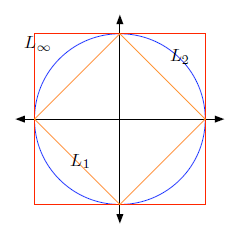
\includegraphics[width=0.3\textwidth]{figures/Lp-distances.png}
        \caption{Comparing the different $L_p$ distances. Adapted from (\cite{phillips_notes}).}
\end{figure}

\end{frame}

\begin{frame}{Distances between metric spaces: Hausdorff and Gromov-Hausdorff distances}
\begin{defn}[Hausdorff distance]
    Suppose $A, B \subseteq X$ are closed sets of the same metric space.
    \begin{align}
        d_H(A, B) =\inf\{\epsilon >0 \mid A\subseteq B^\epsilon \text{ and } B\subseteq A^\epsilon\},
    \end{align}
    where $A^\epsilon$ denotes the $\epsilon$-thickening of $A$.
\end{defn}

\begin{defn}[Gromov-Hausdorff distance]
Suppose $A, B$ are two closed metric spaces (can be distinct).
    \begin{align}
        d_{GH}(A,B) =\inf_{f,g}\{d_H(f_{A\to X}(A), g_{B\to X}(B))\},
    \end{align}
where $f_{A\to X}$ denotes an isometric embedding of $A$ into some metric space $X$ and $f_{B\to X}$ denotes an isometric embedding of $B$ into some metric space $X$. The infimum is taken over all possible such embeddings. 
\end{defn}
\end{frame}
\begin{frame}{Distances between metric spaces: Hausdorff and Gromov-Hausdorff distances}
   \begin{figure}[H]
   \label{matching}
        \centering 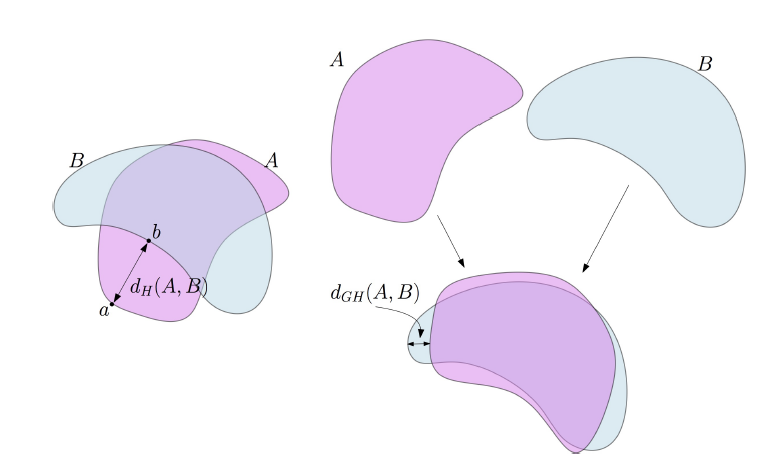
\includegraphics[width=0.8\textwidth]{figures/gomorov-hausdorf.png}
            \caption{Comparison between Hausdorff and Gromov-Hausdorff distances. Adapted from (\cite{chazal_introduction_2021}).}
    \end{figure}
\end{frame}

\begin{frame}{Distances between topological features: Bottleneck distance}
    \begin{defn}[Bottleneck distance]
\begin{align}
    d_B(dgm_1, dgm_2) = \inf_M\{\max_{(x,y)\in M} \|x-y\|_\infty\},
\end{align}
where the infimum is taken over all possible matchings $M$.
\end{defn}
   \begin{figure}[H]
   \label{matching}
        \centering 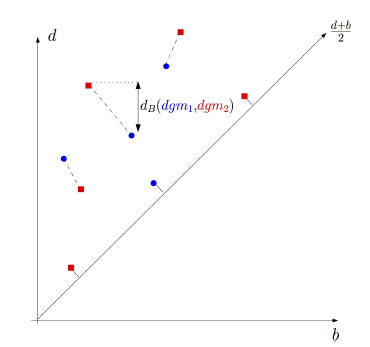
\includegraphics[width=0.3\textwidth]{figures/matching.png}
            \caption{A perfect matching and the Bottleneck distance between the blue and red persistent diagrams. Adapted from (\cite{chazal_introduction_2021}).} \label{fig:perfect-matching}
    \end{figure}
\end{frame}

\begin{frame}{Distances between topological features: distance}
    
\begin{defn}[$p$-Wasserstein distance]
Given $p\geq 1$, the $p$-Wasserstein distance between a pair of persistence diagrams $\dgm_1$ and $\dgm_2$ is defined by 
\begin{align}
    W_p(\dgm_1, \dgm_2) = \left(\inf_M \sum_{(x,y)\in M}\|x-y\|^p_\infty\right)^{1/p},
\end{align}
where the infimum is taken over all possible matchings $M$.
\end{defn}
As $p$ tends to infinity, the Wasserstein distance approaches the bottleneck distance.
\end{frame}
\section{Application}

\begin{frame}{Application to neural data: Data collection}
 \begin{itemize}
        \item Moving visual stimuli of artificial gratings are flashed in front of the mouse.
        \item Each visual stimuli are shifting in 8 directions over time.
        \item Neuron output is recorded with electrodes and encoded in peristimulus (PSTH) diagrams.
        \item Each PSTH diagram shows the firing rate of one neuron over time for 8 directions. Brighter pixels indicate higher firing rates.
    \end{itemize} 
 \begin{figure}[H]
        \centering
            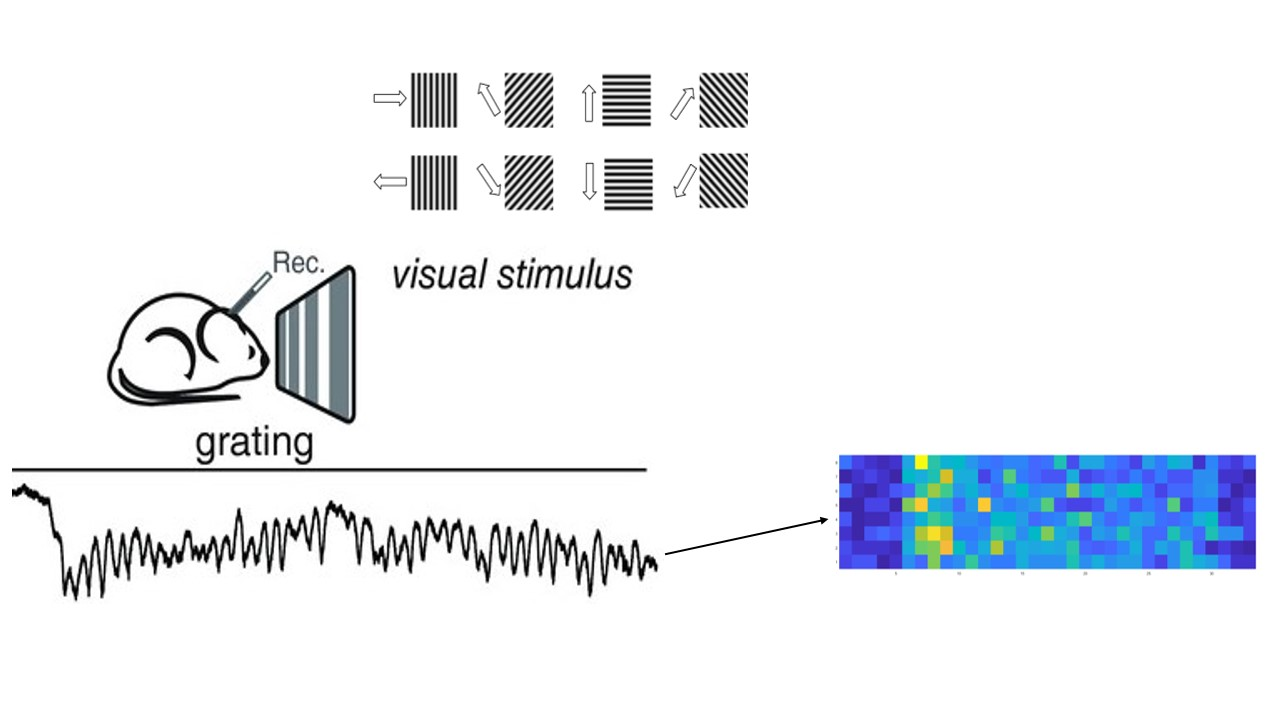
\includegraphics[width=0.55\textwidth]{figures/Slide5.jpg}
            \caption{Visualising neural data from lab experiments.}
    \end{figure}
\end{frame}

\begin{frame}{Neural tensors}
\begin{defn}[Neural population response]
    Suppose $\mathcal{S}$ is a set of $S$ visual stimuli (e.g., images) $\mathcal{S} = \{s_1, s_2,\dots, s_S\}$, each moving over a time interval of $T$ in $d$ directions. The \underline{neural population response} of a set of $N$ neurons to a stimulus $m_i$ over time is $\mathcal{N} = \{\vec{n}_1, \vec{n}_2, \dots, \vec{n}_N\},$ where $\vec{n}_i \in \mathbb{R}^{dT}$. 
\end{defn}
\begin{defn}[Neural tensors]
    Each \underline{neural tensor} encodes the neural population response of a set of neurons to a set of moving visual stimulus over the time and directions of the movement. It is thus a $3$-way tensor of dimension $N$-by-$S$-by-$dT$.
\end{defn}
\end{frame}
\begin{frame}{Build point clouds from neural tensors}
The neural spiking data set used in this project is represented by a $3$-way tensor of dimension $698$-by-$6$-by-$264$, where the dimensions represent: 
\begin{enumerate}
    \item $698$ neurons 
    \item $6$ types of visual stimuli
    \item $264$ number of pixels in the PSTH diagram
\end{enumerate}

Thus we have
\begin{itemize}
    \item Six point clouds each corresponds to the neural population response towards one type of stimuli, which we denote as $X_1, X_2, \dots,X_6$.
    \item Each point cloud $X_i$ consists of $698$ points in $\RR^{264}$. 
\end{itemize}
\end{frame}

\begin{frame}{Step 1 dimensionality reduction: implementation}
    
    \begin{itemize}
        \item The Manifold Hypothesis states that real-world high-dimensional data lie on low-dimensional manifolds embedded within the high-dimensional space. (\cite{deepai_2019})
        \item  Neural spiking data is high-dimensional, but the neural connections constrain the possible patterns of population activity (\cite{okun_diverse_2015}, \cite{sadtler_neural_2014}, \cite{tsodyks_attractor_1999}) and that the possible patterns are confined to a low-dimensional manifold (\cite{stopfer_intensity_2003},  \cite{yu_gaussian-process_2009}).
        \item We reduced the dimensionaltity of each point cloud from the space of $\RR^{264}$ to $\RR^3$ using diffusion map implemented with pydiffmap package (\cite{eastman_pydiffmap_2017})
    \end{itemize}
    \end{frame}
    
    \begin{frame}{Step 1 dimensionality reduction: results}
\begin{figure}[H]
\centering
\begin{subfigure}[b]{0.3\textwidth}
    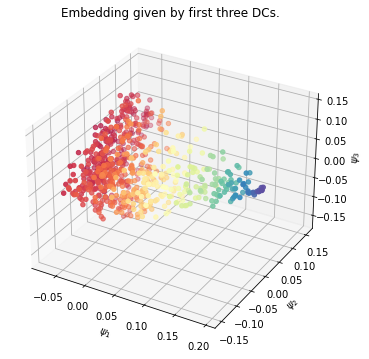
\includegraphics[width=\textwidth]{figures/X1_embedding.png}
    \caption{Three-dimensional embedding of $X_1$.}
\end{subfigure}
\hfill
\begin{subfigure}[b]{0.3\textwidth}
    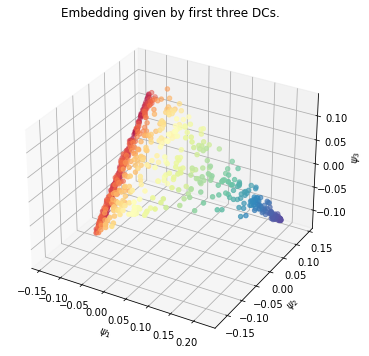
\includegraphics[width=\textwidth]{figures/X2_embedding.png}
    \caption{Three-dimensional embedding of $X_2$.}
\end{subfigure}
\hfill
\begin{subfigure}[b]{0.3\textwidth}
    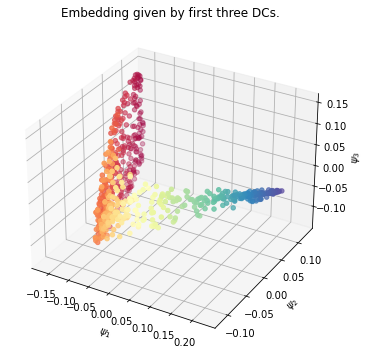
\includegraphics[width=\textwidth]{figures/X3_embedding.png}
    \caption{Three-dimensional embedding of $X_3$.}
\end{subfigure}
\hfill
\begin{subfigure}[b]{0.3\textwidth}
    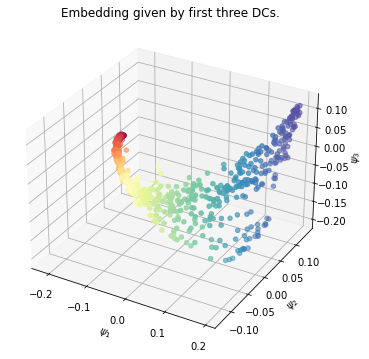
\includegraphics[width=\textwidth]{figures/X4_embedding.png}
    \caption{Three-dimensional embedding of $X_4$.}
\end{subfigure}
\hfill
\begin{subfigure}[b]{0.3\textwidth}
    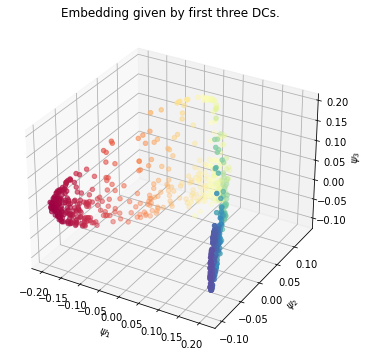
\includegraphics[width=\textwidth]{figures/X5_embedding.png}
    \caption{Three-dimensional embedding of $X_5$.}
\end{subfigure}
\hfill
\begin{subfigure}[b]{0.3\textwidth}
    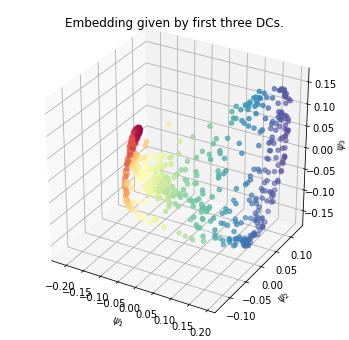
\includegraphics[width=\textwidth]{figures/X6_embedding.png}
    \caption{Three-dimensional embedding of $X_6$.}
\end{subfigure}
\end{figure}
\end{frame}

\begin{frame}{Step 2 persistent homology: implementation}
\begin{itemize}
    \item We applied persistent homology to extract the topological features from the six embeddings respectively.

    \item We used the package ripser (\cite{ctralie2018ripser}) to obtain the respective persistence diagrams from the embeddings.
    
    \item Using the (birth, death)-intervals from each persistence diagram, we then wrote code to draw the equivalent persistence barcode representation.
\end{itemize}
\end{frame}

\begin{frame}{Step 2 persistent homology: results}
\begin{figure}[H]
\centering
\begin{subfigure}[b]{0.2\textwidth}
    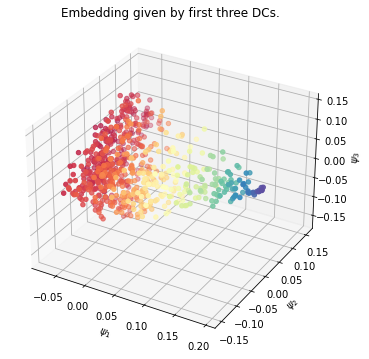
\includegraphics[width=\textwidth]{figures/X1_embedding.png}
    \caption{Three-dimensional embedding of $X_1$.}
\end{subfigure}
\hfill
\begin{subfigure}[b]{0.75\textwidth}
    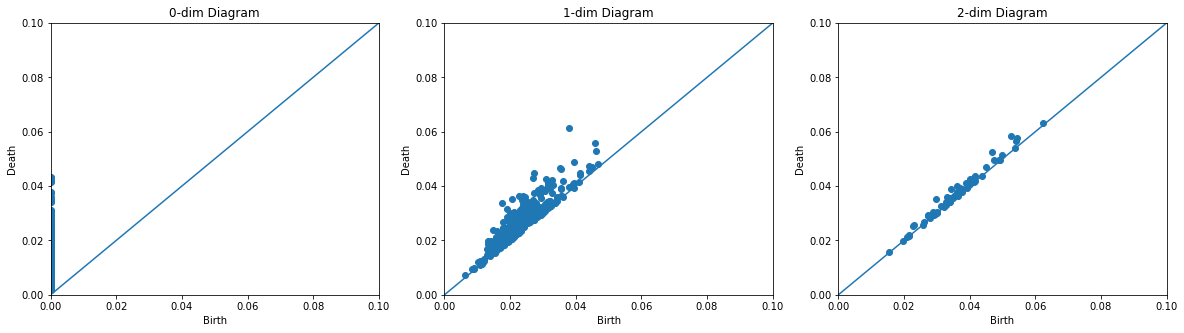
\includegraphics[width=\textwidth]{figures/X1_H0.png}
    \caption{Persistence diagrams.}
\end{subfigure}
\begin{subfigure}[b]{0.25\textwidth}

\includegraphics[width=\textwidth]{figures/white.png} 
\end{subfigure}
\begin{subfigure}[b]{0.2\textwidth}
    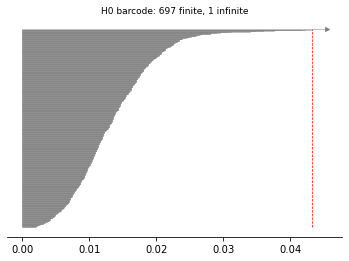
\includegraphics[width=\textwidth]{figures/X1_H0_barcode.png}
    \caption{}
\end{subfigure}
\begin{subfigure}[b]{0.2\textwidth}
    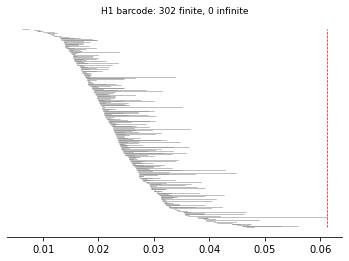
\includegraphics[width=\textwidth]{figures/X1_H1_barcode.png}
        \caption{Persistence barcodes.}
\end{subfigure}
\begin{subfigure}[b]{0.2\textwidth}
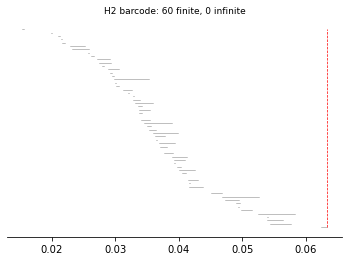
\includegraphics[width=\textwidth]{figures/X1_H2_barcode.png}
 \caption{}
\end{subfigure}
\caption{Results for applying persistent homology on the three-dimensional embedding of $X_1$.}
\end{figure}
\end{frame}

\begin{frame}{Step 2 persistent homology: results}
\begin{figure}[H]
\centering
\begin{subfigure}[b]{0.2\textwidth}
    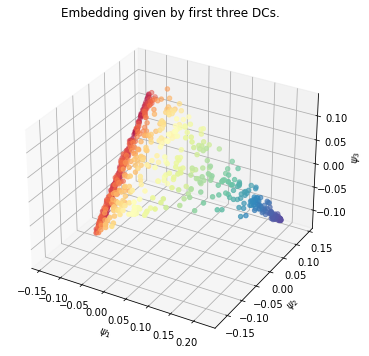
\includegraphics[width=\textwidth]{figures/X2_embedding.png}
    \caption{Three-dimensional embedding of $X_2$.}
\end{subfigure}
\hfill
\begin{subfigure}[b]{0.75\textwidth}
    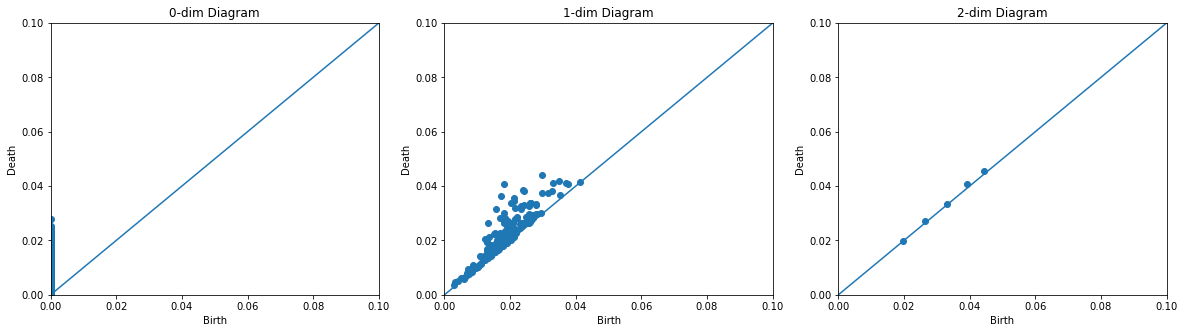
\includegraphics[width=\textwidth]{figures/X2_H0.png}
    \caption{Persistence diagrams.}
\end{subfigure}
\begin{subfigure}[b]{0.25\textwidth}

\includegraphics[width=\textwidth]{figures/white.png} 
\end{subfigure}
\begin{subfigure}[b]{0.2\textwidth}
    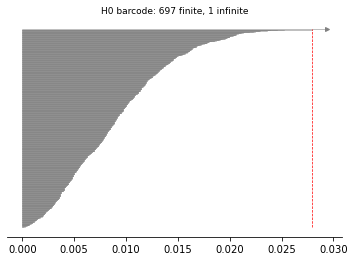
\includegraphics[width=\textwidth]{figures/X2_H0_barcode.png}
    \caption{}
\end{subfigure}
\begin{subfigure}[b]{0.2\textwidth}
    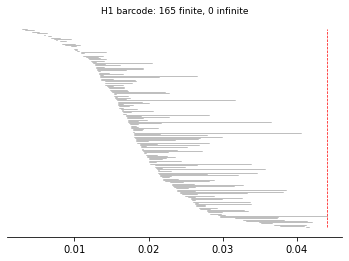
\includegraphics[width=\textwidth]{figures/X2_H1_barcode.png}
        \caption{Persistence barcodes.}
\end{subfigure}
\begin{subfigure}[b]{0.2\textwidth}
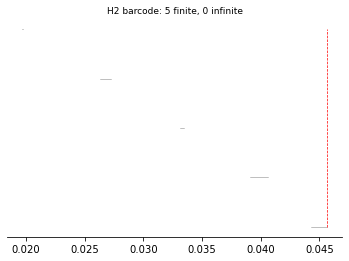
\includegraphics[width=\textwidth]{figures/X2_H2_barcode.png}
 \caption{}
\end{subfigure}
\caption{Results for applying persistent homology on the three-dimensional embedding of $X_2$.}
\end{figure}
\end{frame}
\begin{frame}{Step 2 persistent homology: results}
\begin{figure}[H]
\centering
\begin{subfigure}[b]{0.2\textwidth}
    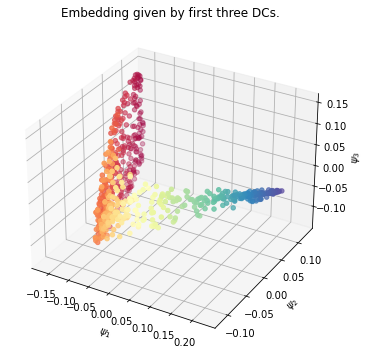
\includegraphics[width=\textwidth]{figures/X3_embedding.png}
    \caption{Three-dimensional embedding of $X_3$.}
\end{subfigure}
\hfill
\begin{subfigure}[b]{0.75\textwidth}
    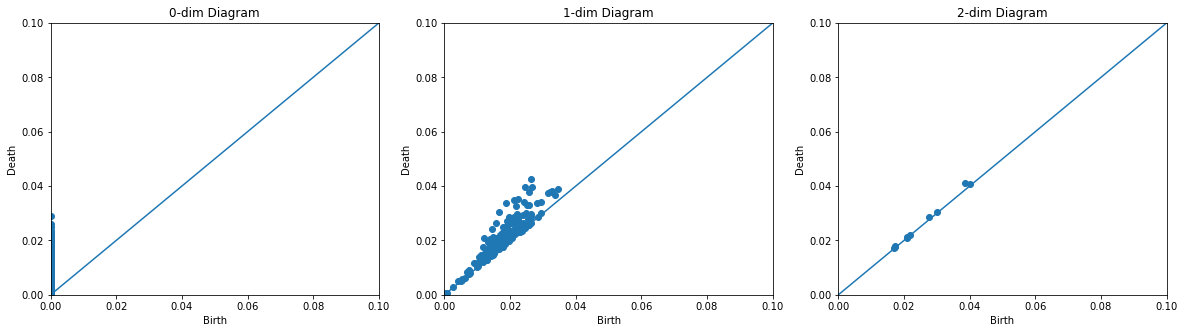
\includegraphics[width=\textwidth]{figures/X3_H0.png}
    \caption{Persistence diagrams.}
\end{subfigure}
\begin{subfigure}[b]{0.25\textwidth}

\includegraphics[width=\textwidth]{figures/white.png} 
\end{subfigure}
\begin{subfigure}[b]{0.2\textwidth}
    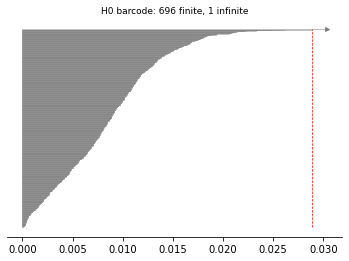
\includegraphics[width=\textwidth]{figures/X3_H0_barcode.png}
    \caption{}
\end{subfigure}
\begin{subfigure}[b]{0.2\textwidth}
    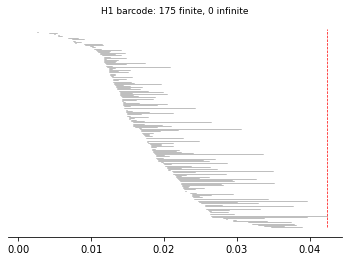
\includegraphics[width=\textwidth]{figures/X3_H1_barcode.png}
        \caption{Persistence barcodes.}
\end{subfigure}
\begin{subfigure}[b]{0.2\textwidth}
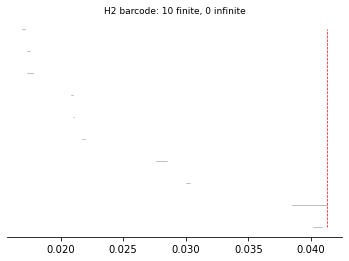
\includegraphics[width=\textwidth]{figures/X3_H2_barcode.png}
 \caption{}
\end{subfigure}
\caption{Results for applying persistent homology on the three-dimensional embedding of $X_3$.}
\end{figure}
\end{frame}
\begin{frame}{Step 2 persistent homology: results}
\begin{figure}[H]
\centering
\begin{subfigure}[b]{0.2\textwidth}
    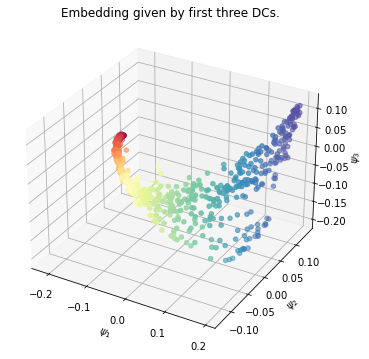
\includegraphics[width=\textwidth]{figures/X4_embedding.png}
    \caption{Three-dimensional embedding of $X_4$.}
\end{subfigure}
\hfill
\begin{subfigure}[b]{0.75\textwidth}
    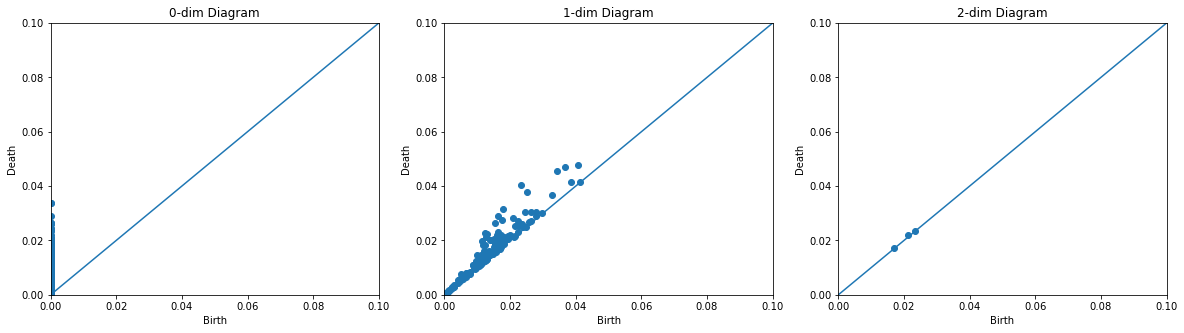
\includegraphics[width=\textwidth]{figures/X4_H0.png}
    \caption{Persistence diagrams.}
\end{subfigure}
\begin{subfigure}[b]{0.25\textwidth}

\includegraphics[width=\textwidth]{figures/white.png} 
\end{subfigure}
\begin{subfigure}[b]{0.2\textwidth}
    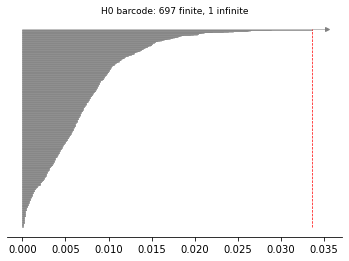
\includegraphics[width=\textwidth]{figures/X4_H0_barcode.png}
    \caption{}
\end{subfigure}
\begin{subfigure}[b]{0.2\textwidth}
    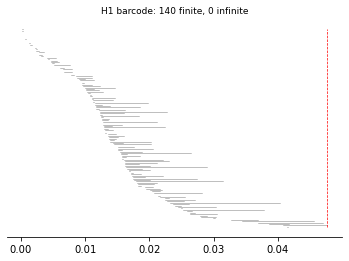
\includegraphics[width=\textwidth]{figures/X4_H1_barcode.png}
        \caption{Persistence barcodes.}
\end{subfigure}
\begin{subfigure}[b]{0.2\textwidth}
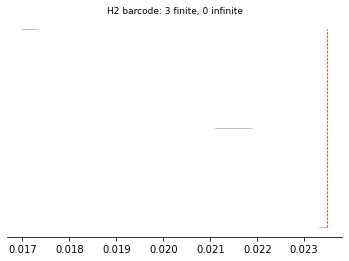
\includegraphics[width=\textwidth]{figures/X4_H2_barcode.png}
 \caption{}
\end{subfigure}
\caption{Results for applying persistent homology on the three-dimensional embedding of $X_4$.}
\end{figure}
\end{frame}
\begin{frame}{Step 2 persistent homology: results}
\begin{figure}[H]
\centering
\begin{subfigure}[b]{0.2\textwidth}
    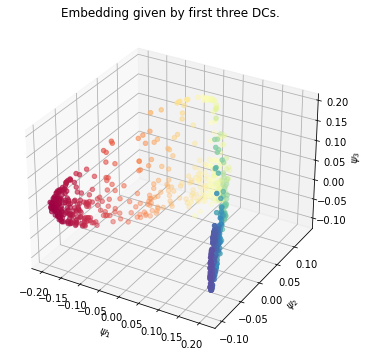
\includegraphics[width=\textwidth]{figures/X5_embedding.png}
    \caption{Three-dimensional embedding of $X_5$.}
\end{subfigure}
\hfill
\begin{subfigure}[b]{0.75\textwidth}
    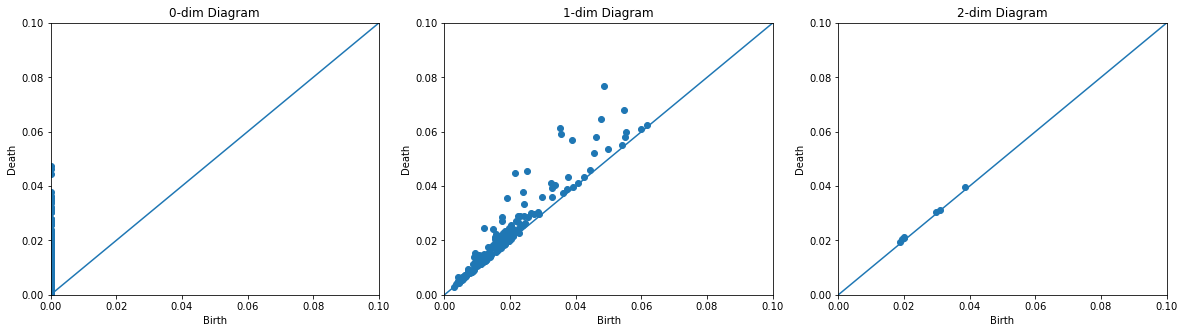
\includegraphics[width=\textwidth]{figures/X5_H0.png}
    \caption{Persistence diagrams.}
\end{subfigure}
\begin{subfigure}[b]{0.25\textwidth}

\includegraphics[width=\textwidth]{figures/white.png} 
\end{subfigure}
\begin{subfigure}[b]{0.2\textwidth}
    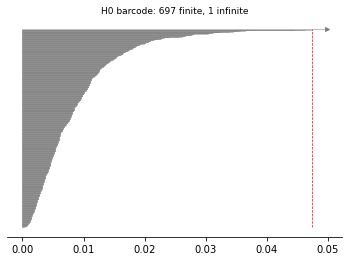
\includegraphics[width=\textwidth]{figures/X5_H0_barcode.png}
    \caption{}
\end{subfigure}
\begin{subfigure}[b]{0.2\textwidth}
    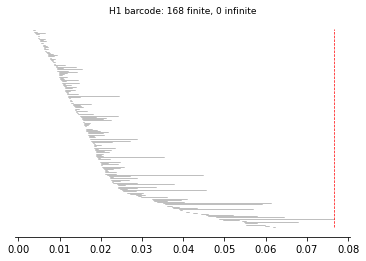
\includegraphics[width=\textwidth]{figures/X5_H1_barcode.png}
        \caption{Persistence barcodes.}
\end{subfigure}
\begin{subfigure}[b]{0.2\textwidth}
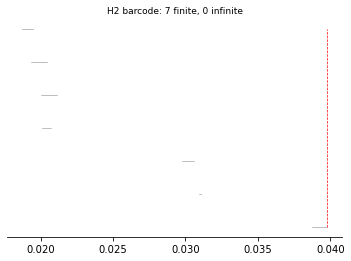
\includegraphics[width=\textwidth]{figures/X5_H2_barcode.png}
 \caption{}
\end{subfigure}
\caption{Results for applying persistent homology on the three-dimensional embedding of $X_5$.}
\end{figure}
\end{frame}
\begin{frame}{Step 2 persistent homology: results}
\begin{figure}[H]
\centering
\begin{subfigure}[b]{0.2\textwidth}
    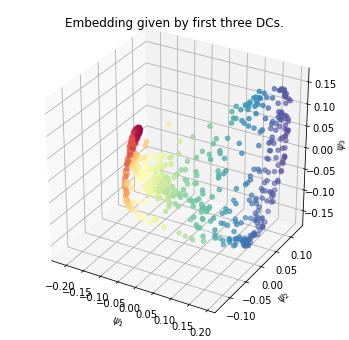
\includegraphics[width=\textwidth]{figures/X6_embedding.png}
    \caption{Three-dimensional embedding of $X_6$.}
\end{subfigure}
\hfill
\begin{subfigure}[b]{0.75\textwidth}
    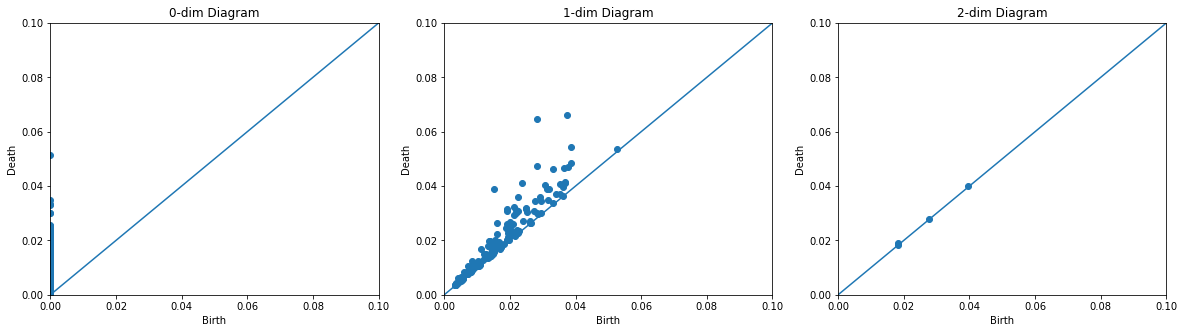
\includegraphics[width=\textwidth]{figures/X6_H0.png}
    \caption{Persistence diagrams.}
\end{subfigure}
\begin{subfigure}[b]{0.25\textwidth}

\includegraphics[width=\textwidth]{figures/white.png} 
\end{subfigure}
\begin{subfigure}[b]{0.2\textwidth}
    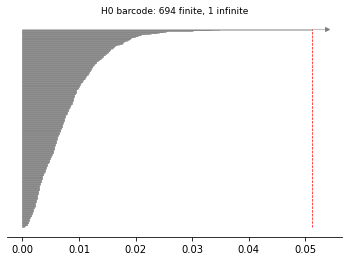
\includegraphics[width=\textwidth]{figures/X6_H0_barcode.png}
    \caption{}
\end{subfigure}
\begin{subfigure}[b]{0.2\textwidth}
    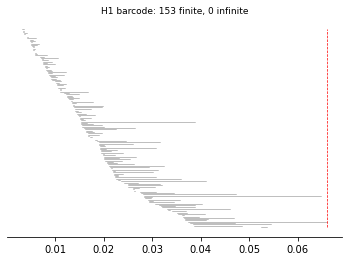
\includegraphics[width=\textwidth]{figures/X6_H1_barcode.png}
        \caption{Persistence barcodes.}
\end{subfigure}
\begin{subfigure}[b]{0.2\textwidth}
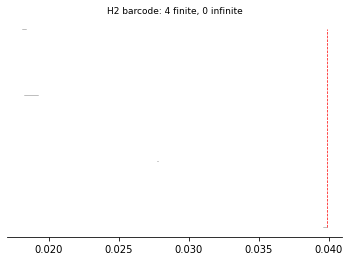
\includegraphics[width=\textwidth]{figures/X6_H2_barcode.png}
 \caption{}
\end{subfigure}
\caption{Results for applying persistent homology on the three-dimensional embedding of $X_6$.}
\end{figure}
\end{frame}

\begin{frame}{Step 3 $p$-Wasserstein distance: results}
In the last step, we used the gudhi package (\cite{gudhi:urm}) to compute the pairwise Wasserstein distance between the persistence diagrams. The method used is based on (\cite{kerber_geometry_2016}). 
\begin{table}[!htbp]
        \centering
        \small
        \setlength\tabcolsep{5pt}
        \begin{tabular}{|c|c|c|c|c|c|c|}
\hline
 $H_0$& $X_1$ & $X_2$ & $X_3$ & $X_4$ & $X_5$ & $X_6$\\
 \hline
$X_1$ &
0.0&
2.77&
3.05&
3.95&
3.08&
3.42
\\
\hline
$X_2$ &
2.77&
0.0&
0.43&
1.35&
1.0&
0.84
\\
\hline
$X_3$ &
3.05&
0.43&
0.0&
1.03&
0.94&
0.66
\\
\hline
$X_4$ &
3.95&
1.35&
1.03&
0.0&
1.11&
0.72
\\
\hline
$X_5$ &
3.08&
1.0&
0.94&
1.11&
0.0&
0.51
\\
\hline
$X_6$ &
3.42&
0.84&
0.66&
0.72&
0.51&
0.0
\\
\hline
\end{tabular}
\caption{Pairwise Wasserstein distance between persistent diagrams for homology group $H_0$.}
\label{tab:Wass_H0}
\end{table}
\end{frame}

\begin{frame}{Step 3 $p$-Wasserstein distance: results}
\begin{table}[!htbp]
        \centering
        \small
        \setlength\tabcolsep{5pt}
        \begin{tabular}{|c|c|c|c|c|c|c|}
\hline
 $H_1$& $X_1$ & $X_2$ & $X_3$ & $X_4$ & $X_5$ & $X_6$ \\ \hline
$X_1$ &
0.0&
0.46&
0.5&
0.64&
0.64&
0.55

\\\hline
$X_2$ &
0.46&
0.0&
0.17&
0.29&
0.36&
0.3
\\\hline
$X_3$ &
0.5&
0.17&
0.0&
0.25&
0.33&
0.3
\\\hline 
$X_4$ &
0.64&
0.29&
0.25&
0.0&
0.27&
0.29
\\\hline 
$X_5$ &
0.64&
0.36&
0.33&
0.27&
0.0&
0.26

\\\hline
$X_6$ &
0.55&
0.3&
0.3&
0.29&
0.26&
0.0\\
\hline
\end{tabular}
\caption{Pairwise Wasserstein distance between persistent diagrams for homology group $H_1$.}
\label{tab:Wass_H1}
\end{table}
\end{frame}

\begin{frame}{Step 3 $p$-Wasserstein distance: results}
\begin{table}[!htbp]
        \centering
        \small
        \setlength\tabcolsep{5pt}
        \begin{tabular}{|c|c|c|c|c|c|c|}
\hline
 $H_2$& $X_1$ & $X_2$ & $X_3$ & $X_4$ & $X_5$ & $X_6$ \\ \hline
$X_1$ &
0.0&
0.06&
0.06&
0.06&
0.06&
0.06
\\
\hline
$X_2$ &
0.06&
0.0&
0.01&
0.0&
0.01&
0.0
\\
\hline
$X_3$ &
0.06&
0.01&
0.0&
0.0&
0.01&
0.0
\\
\hline
$X_4$ &
0.06&
0.0&
0.0&
0.0&
0.0&
0.0
\\
\hline
$X_5$ &
0.06&
0.01&
0.01&
0.0&
0.0&
0.0
\\
\hline
$X_6$ &
0.06&
0.0&
0.0&
0.0&
0.0&
0.0
\\
\hline
\end{tabular}
\caption{Pairwise Wasserstein distance between persistent diagrams for homology group $H_2$.}
\label{tab:Wass_H2}
\end{table}
\end{frame}

\begin{frame}{Extension: comparison with known shapes ($2$-sphere)}
    \begin{figure}[H]
\centering
\begin{subfigure}[b]{0.2\textwidth}
    \includegraphics[width=\textwidth]{figures/dsphere.png}
    \caption{Scatter plot for $2$-sphere.}
\end{subfigure}
\hfill
\begin{subfigure}[b]{0.75\textwidth}
    \includegraphics[width=\textwidth]{figures/dsphere_Hk.png}
    \caption{Persistence diagrams.}
\end{subfigure}
\begin{subfigure}[b]{0.25\textwidth}
\includegraphics[width=\textwidth]{figures/white.png} 
\end{subfigure}
\begin{subfigure}[b]{0.2\textwidth}
    \includegraphics[width=\textwidth]{figures/dsphere_H0_barcode.png}
    \caption{}
\end{subfigure}
\begin{subfigure}[b]{0.2\textwidth}
    \includegraphics[width=\textwidth]{figures/dsphere_H1_barcode.png}
        \caption{Persistence barcodes.}
\end{subfigure}
\begin{subfigure}[b]{0.2\textwidth}
\includegraphics[width=\textwidth]{figures/dsphere_H2_barcode.png}
 \caption{}
\end{subfigure}
\caption{Results for applying persistent homology on the $2$-sphere.}
\end{figure}
\end{frame}

\begin{frame}{Extension: comparison with known shapes (torus)}
\begin{figure}[H]
\centering
\begin{subfigure}[b]{0.2\textwidth}
    \includegraphics[width=\textwidth]{figures/torus.png}
    \caption{Scatter plot for the three-dimensional torus.}
\end{subfigure}
\hfill
\begin{subfigure}[b]{0.75\textwidth}
    \includegraphics[width=\textwidth]{figures/torus_Hk.png}
    \caption{Persistence diagrams.}
\end{subfigure}
\begin{subfigure}[b]{0.25\textwidth}
\includegraphics[width=\textwidth]{figures/white.png} 
\end{subfigure}
\begin{subfigure}[b]{0.2\textwidth}
    \includegraphics[width=\textwidth]{figures/torus_H0_barcode.png}
    \caption{}
\end{subfigure}
\begin{subfigure}[b]{0.2\textwidth}
    \includegraphics[width=\textwidth]{figures/torus_H1_barcode.png}
        \caption{Persistence barcodes.}
\end{subfigure}
\begin{subfigure}[b]{0.2\textwidth}
\includegraphics[width=\textwidth]{figures/torus_H2_barcode.png}
 \caption{}
\end{subfigure}
\caption{Results for applying persistent homology on the three-dimensional torus.}
\end{figure}
\end{frame}

\begin{frame}{Extension: comparison with known shapes ($p$-Wasserstein distance)}

Then, we computed the Wasserstein distance between the six point clouds and the known shapes:

\begin{table}[!htbp]
        \centering
        \small
        \setlength\tabcolsep{5pt}
        \begin{tabular}{|c|c|c|c|c|c|c|}
\hline
  $H_0$& $X_1$ & $X_2$ & $X_3$ & $X_4$ & $X_5$ & $X_6$ \\ \hline
$2$-sphere & 2.48 & 4.46&  4.64 & 5.18 & 4.53 & 4.83\\\hline
torus & 3.63 &  1.46 & 1.31 & 0.73 & 1.38 & 1.06 \\ \hline
\end{tabular}
\end{table}


\begin{table}[!htbp]
        \centering
        \small
        \setlength\tabcolsep{5pt}
        \begin{tabular}{|c|c|c|c|c|c|c|}
\hline
$H_1$& $X_1$ & $X_2$ & $X_3$ & $X_4$ & $X_5$ & $X_6$ \\ \hline
$2$-sphere & 0.62 &   0.77 & 0.80 & 0.87 & 0.85 & 0.76\\\hline
torus & 0.74 & 0.49 & 0.44 & 0.34 & 0.45 & 0.47\\ \hline
\end{tabular}
\end{table}

\begin{table}[!htbp]
        \centering
        \small
        \setlength\tabcolsep{5pt}
        \begin{tabular}{|c|c|c|c|c|c|c|}
\hline
$H_2$ & $X_1$ & $X_2$ & $X_3$ & $X_4$ & $X_5$ & $X_6$ \\ \hline
$2$-sphere & 0.11 &   0.12 & 0.12 & 0.12 & 0.13 & 0.12\\\hline
torus & 0.057 & 0.017 & 0.018  & 0.016 & 0.018 & 0.016 \\ \hline
\end{tabular}
\end{table}
\end{frame}

\section{Conclusion}

\begin{frame}{Analysis of results}
    Based on the results from the above tables of Wasserstein distances, our observations and inferences are as follows.

\begin{enumerate}
    \item Neural population response evoked by stimulus type 1 is significantly different from the other stimulus types. 
    
    \item The intrinsic dimensionality of this neural data might be even lower than three-dimensional since there is no significant differences in homology groups $H_2$ for the point clouds.
    
    \item The topological structure of the neural population response evoked by stimuli type 1 is more similar to a sphere while those evoked by the other stimuli types are more similar to a torus. 
    
    % It would be interesting to compare this result with the hypothesis in (\cite{ben-yishai_theory_1995}, \cite{Blumenfeld_2006}, \cite{goldberg_randomized_2004},    \cite{singh_top_v1_2008}):
    % If we are given an oriented stimulus, and if the orientation is a circular variable, then the hypothesis is that the neural population response evoked by such stimulus must have a topological structure equivalent to that of a circle. However, to fully test this hypothesis, further experiments with different types of stimuli need to be conducted.
\end{enumerate}
\end{frame}

\begin{frame}{Conclusions}
\begin{itemize}
    \item In this project, we proposed a topological approach to compare high-dimensional point clouds and provided a concrete application to neural spiking data. 
    \item Limitations: lab data involve sampling errors such as missing data and inconsistent densities, causing noise to the true underlying geometry of the neural population response.
    \item Advantages: our approach obtained a useful summary of the global geometric structure of the neural spiking data in terms of how similarly the neurons collectively respond to visual stimuli.
    % \item As an emerging field, TDA will certainly see more applications in solving problems that involve understanding the geometric and topological structure of high-dimensional data.
\end{itemize}
\end{frame}

\begin{frame}{Acknowledgements}
I would like to thank my mentor Prof.~Han Fei for his continual support throughout the project. There have been ups and downs in this project, but Prof.~Han Fei has helped me stay flexible and keep a keen spirit for learning and discovery. I am also grateful for support from my family and friends.
\end{frame}
\section{References}
\frametitle{bibliography}
\printbibliography[heading=bibintoc]
\end{document}